\documentclass{article}
\usepackage{color}
\definecolor{lightgray}{rgb}{0.95, 0.95, 0.95}
\definecolor{darkgray}{rgb}{0.4, 0.4, 0.4}
%\definecolor{purple}{rgb}{0.65, 0.12, 0.82}
\definecolor{editorGray}{rgb}{0.95, 0.95, 0.95}
\definecolor{editorOcher}{rgb}{1, 0.5, 0} % #FF7F00 -> rgb(239, 169, 0)
\definecolor{editorGreen}{rgb}{0, 0.5, 0} % #007C00 -> rgb(0, 124, 0)
\definecolor{orange}{rgb}{1,0.45,0.13}		
\definecolor{olive}{rgb}{0.17,0.59,0.20}
\definecolor{brown}{rgb}{0.69,0.31,0.31}
\definecolor{purple}{rgb}{0.38,0.18,0.81}
\definecolor{lightblue}{rgb}{0.1,0.57,0.7}
\definecolor{lightred}{rgb}{1,0.4,0.5}
\usepackage{upquote}
\usepackage{listings}
%python
\lstdefinestyle{py} {%
language=python,
literate=%
*{0}{{{\color{lightred}0}}}1
{1}{{{\color{lightred}1}}}1
{2}{{{\color{lightred}2}}}1
{3}{{{\color{lightred}3}}}1
{4}{{{\color{lightred}4}}}1
{5}{{{\color{lightred}5}}}1
{6}{{{\color{lightred}6}}}1
{7}{{{\color{lightred}7}}}1
{8}{{{\color{lightred}8}}}1
{9}{{{\color{lightred}9}}}1,
basicstyle=\footnotesize\ttfamily, % Standardschrift
numbers=left,               % Ort der Zeilennummern
%numberstyle=\tiny,          % Stil der Zeilennummern
%stepnumber=2,               % Abstand zwischen den Zeilennummern
numbersep=5pt,              % Abstand der Nummern zum Text
tabsize=4,                  % Groesse von Tabs
extendedchars=true,         %
breaklines=true,            % Zeilen werden Umgebrochen
keywordstyle=\color{blue}\bfseries,
frame=b,
commentstyle=\color{brown}\itshape,
stringstyle=\color{editorOcher}\ttfamily, % Farbe der String
showspaces=false,           % Leerzeichen anzeigen ?
showtabs=false,             % Tabs anzeigen ?
xleftmargin=17pt,
framexleftmargin=17pt,
framexrightmargin=5pt,
framexbottommargin=4pt,
%backgroundcolor=\color{lightgray},
showstringspaces=false,      % Leerzeichen in Strings anzeigen ?
}%








\usepackage{float}
\usepackage{graphicx}
\usepackage{caption}
\usepackage{subcaption}



\begin{document}
\title{Report: Different Sorting Algorithms}
\author{Wenhui Guo, Zhuojun Huang}
\maketitle


\subsection*{Abstract}
This is a report for project 1 in ECE 590. Here, we show our way to implement different sorting algorithms taught in class using Python and make analysis on the algorithms using testing results.

\subsection*{Introduction}
%why sorting
%sorting applications
%briefly introduce different sorting algorithms
%best runtime
In this project, we implemented five algorithms for sorting problem. A sorting algorithm should take a list of elements and put them in a certain order. In this case, we simply sort a list of integers in ascending order. We tried selection sort, insertion sort, bubble sort, merge sort and quicksort, in both small input size and large input size.
In the methods part, we provide the theoretical run times and code implementation for each algorithm. The theoretical runtimes usually measure the time complexity of asymptotically large inputs to measure the bounds of time complexity. The reason we are using theoretical runtime is that we would like to measure the time complexity of an algorithm in a machine-independent way. If we analyze in actual runtimes, the time complexity will largely depend on the architecture and computational resource of a certain machine. For example, quicksort and bubble sort will take almost the same time on a super computer while the results may differ largely if we run them on an old slow machine. Theoretical runtime, on the other hand, won’t bother us in this case. Although in special occasions, we may prefer measuring in actual runtimes to make sure the algorithms run fast on a target machine, this is not general cases and theoretical runtime is the natural choice if we would like to measure time complexity in most cases. 
We implement these five sorting algorithms in python and our results indicate the relationship between input size and actual runtime across our algorithms. And the results reveal that our sorting algorithms work well both unsorted and sorted input arrays. Then we discuss runtime performance of our algorithms.

\newpage

\subsection*{Methods}
%ideas behind different sorting algorithms
%how to implement in python

\subsubsection*{Selection Sort, Time Complexity $O(N^2)$}
\begin{lstlisting}[style = py]
"""
SelectionSort
"""
def SelectionSort(A):
 for i in range(len(A)):      #Loop through the array
       index=i                #sorted part index
       for j in range(i+1,len(A)):    #iterativly go through unsorted part
           if A[index]>A[j]:      
               index=j    #found the element less than sorted, 
                          #\put it in the sorted part
       A[i],A[index]=A[index],A[i]
 return A
\end{lstlisting}

\subsubsection*{Insertion Sort, Time Complexity $O(N^2)$}
\begin{lstlisting}[style = py]
"""
InsertionSort
"""
def InsertionSort(A):
 for i in range(1,len(A)):     #go through the array
        current = A[i]         #sorted part
        for j in range(i-1, -2, -1):    #iterativly go through unsorted part
            if(j == -1 or A[j] <= current): break
            else:
                A[j+1] = A[j]    #swoop over
        A[j+1] = current         #store in sorted part
 return A
\end{lstlisting}

\newpage
\subsubsection*{Bubble Sort, Time Complexity $O(N^2)$}
\begin{lstlisting}[style = py]
"""
BubbleSort
"""
def BubbleSort(A):
 for i in range(0,len(A)):    
        for j in range(i+1,len(A)):   
            if A[i]>A[j]:           #if first element bigger than latter element
                A[i],A[j]=A[j],A[i]    #swap
 return A

\end{lstlisting}

\subsubsection*{Merge Sort, Time Complexity $O(Nlog(N))$}
\begin{lstlisting}[style = py]
'''
MergeSort Helper function
To combine two sorted array together
'''

def CombineTwoSortedArray(A1, A2, A):
    k = 0
    i = 0
    j = 0
    while (i < len(A1) and j < len(A2)): #compare for the smaller one to add in A
        if(A1[i] <= A2[j]):
            A[k] = A1[i]
            i += 1
        elif(A2[j] < A1[i]):
            A[k] = A2[j]
            j += 1
        k += 1

    if(j < len(A2)):   #if all elements in A1 have all in A, 
                       #\put the rest of A2 in A
        A[k:] = A2[j:]
    if(i < len(A1)):   #vice versa
        A[k:] = A1[i:]
    return A
"""
MergeSort

Recursion:
base case:
if length of A==1 or length of A==2

each time n->2*(n/2) plus merge two sorted together
"""
def MergeSort(A):
    if len(A) <= 1:   #base case 1
        return A
    elif len(A) == 2:  #base case 2
        if A[0] > A[1]:
            A[0], A[1] = A[1], A[0]
        return A
    else:
        middle = math.floor(len(A) / 2)  
        A1 = MergeSort(A[0: middle])     #recursive call
        A2 = MergeSort(A[middle: len(A)])
        CombineTwoSortedArray(A1, A2, A)  #combine two sorted part together
        return A



\end{lstlisting}

\subsubsection*{QuickSort, Time Complexity $O(Nlog(N))$}
\begin{lstlisting}[style = py]
"""
QuickSort

Sort a list A with the call QuickSort(A, 0, len(A)).

base case: 
if length==1, issorted

an array A in range [i, j)
pivotIndex, pivotValue
reorganize array A, so that we find the place of the pivotValue, 
i.e every left element of the pivotValue is smaller, right larger
"""
def QuickSort(A, i, j):
    if ((j - i) <= 1): return A    #base case

    pivot = A[i]   
    left = i + 1
    right = j - 1

    while (left <= right):
        while (left <= right and A[left] <= pivot): left += 1 
        #left part: all smaller than or equal to pivotValue, move to the right
        while (A[right] > pivot): right -= 1
        #right part: all bigger than pivotValue, move to the left
        if (left < right):    
            A[left], A[right] = A[right], A[left]  #swap 
              #\since at this time A[left] bigger than pivot 
              #\while A[right] smaller or equal to pivot
    A[i], A[left - 1] = A[left - 1], A[i]  #place pivot in the right place
    QuickSort(A, i, left - 1)  #recursive call
    QuickSort(A, left, j)
    return A
\end{lstlisting}

\subsection*{Results}
\begin{figure}[H]
	\centering
	\begin{subfigure}{.3\textwidth}
		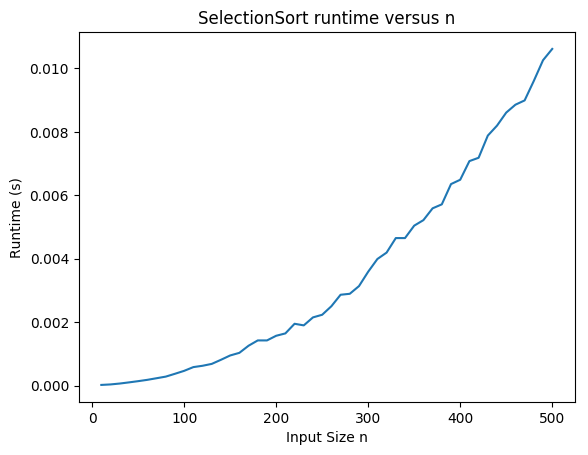
\includegraphics[width=\textwidth]{../results/normal/SelectionSort.png}
		\caption{Selection Sort}
	\end{subfigure}
%%%%%%%%%%%%%%
	\begin{subfigure}{.3\textwidth}
		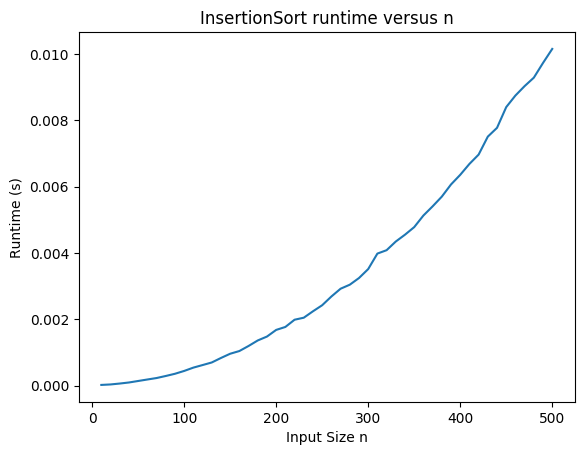
\includegraphics[width=\textwidth]{../results/normal/InsertionSort.png}
		\caption{Insertion Sort}
	\end{subfigure}
%%%%%%%%%%%%%%
	\begin{subfigure}{.3\textwidth}
		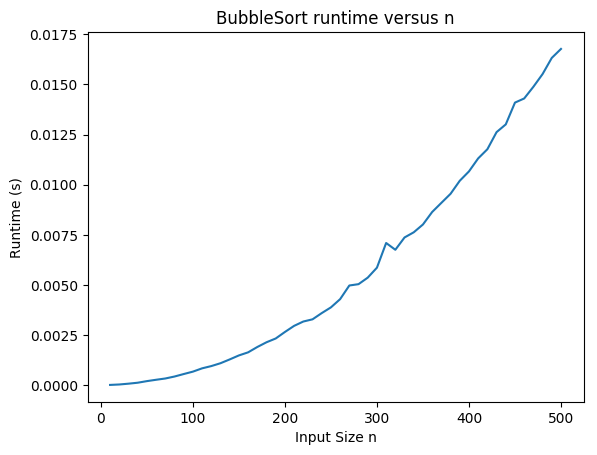
\includegraphics[width=\textwidth]{../results/normal/BubbleSort.png}
		\caption{Bubble Sort}
	\end{subfigure}
	\caption*{}
\end{figure}




\begin{figure}[H]
	\centering
	\begin{subfigure}{.3\textwidth}
		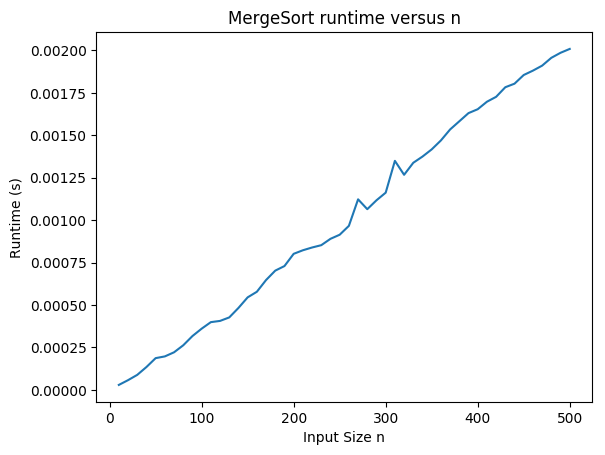
\includegraphics[width=\textwidth]{../results/normal/MergeSort.png}
		\caption{Merge Sort}
	\end{subfigure}
%%%%%%%%%%%%%%
	\begin{subfigure}{.3\textwidth}
		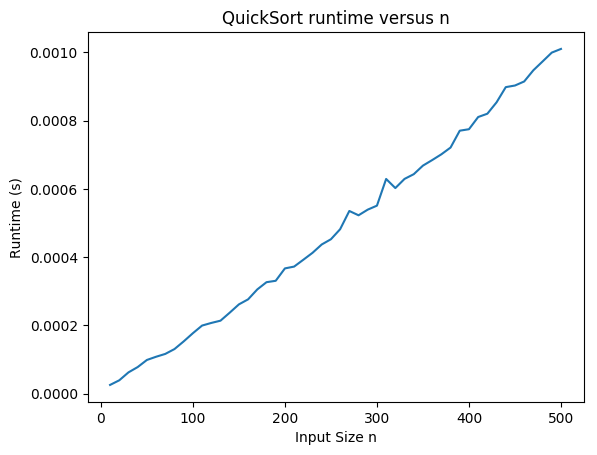
\includegraphics[width=\textwidth]{../results/normal/QuickSort.png}
		\caption{QuickSort}
	\end{subfigure}
%%%%%%%%%%%%%%
	\begin{subfigure}{.3\textwidth}
		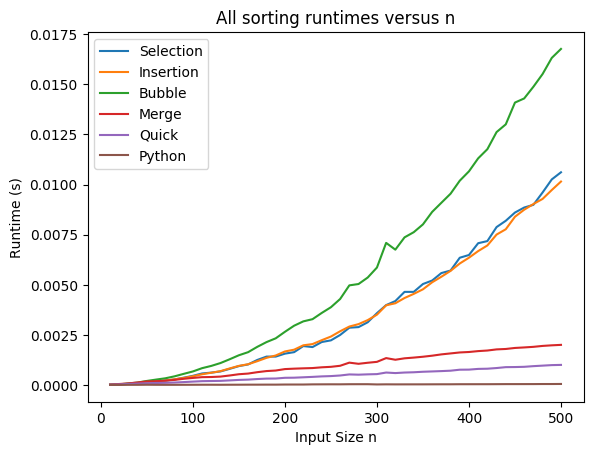
\includegraphics[width=\textwidth]{../results/normal/sorting.png}
		\caption{All Sorting Alg}
	\end{subfigure}
	\caption*{Results}
\end{figure}



\subsection*{Discussion}
\paragraph{THE WAY WE TEST}
For each algorithm, the testing code averaged the actual runtime across multiple trials in different sizes. The reason we are averaging on multiple trials instead of one trial is that in some special cases, some algorithms will run faster than others. But that doesn’t mean they will behave in the same way for more general cases. For example, insertion sort will run faster than the other sorting algorithms in the case of the given input is already sorted. For another example, bubble sort will perform as good as quick sort if the input is in a ascending order. (if the quick sort algorithm doesn’t apply randomized method).

\begin{figure}[H]
\centering
	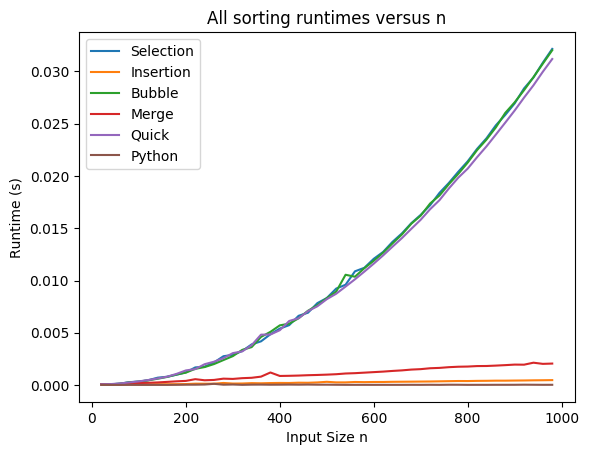
\includegraphics[width = \textwidth]{../results/one_trial}
	\caption{Testing algorithms with one trial}
\end{figure}
Above is the result of running all the sorting algorithms with one trial, where our input array is already sorted. It will be tempting to conclude that merge sort and insertion sort are better than any other algorithms regarding the result we get. However, it is not true because insertion sort only works well in the case that its input list is already sorted. Multiple trials on our algorithms will reduce the probability for such events happened.


For all these five sorting algorithms, no matter the input is sorted or unsorted, the output behaves as expected to produce a sorted array. And according to the runtime picture, we can conclude that quicksort takes the least time to sort an array while bubble sort takes the most time. However, the actual result appears to be contradict to what we addressed in class that the time complexities of bubble sort and selection sort are the same. In real world, the bubble sort takes more time than selection sort. The reason is that bubble sort requires more swap operations each iteration, which result in longer time. 
\paragraph{ALGORITHMS COMPARISON}
Among these algorithms, we think that quicksort is the best and Bubble sort is the worst. According to the runtimes of all algorithms, it is clearly that quick sort is best since it has the least runtime, and bubble sort is the worst because the runtime is way larger than the else.
I think it is because bubble sort always requires $O(N^2)$ times, and requires more “swap” operations than selection sort, which requires only N times.

\paragraph{INPUT SIZE}
For the small value of n, the runtimes of all algorithms appear to be relevantly close. Because with small input size $N$, algorithms of $O(N^2)$and $O(Nlog(N)) $only have subtle difference.

\paragraph{Machine Environment}
In addition, we test all these algorithms without expensive computational tasks in the background. If we do have expensive tasks in the background, the result will behave abnormally.
\begin{figure}[H]
\centering
	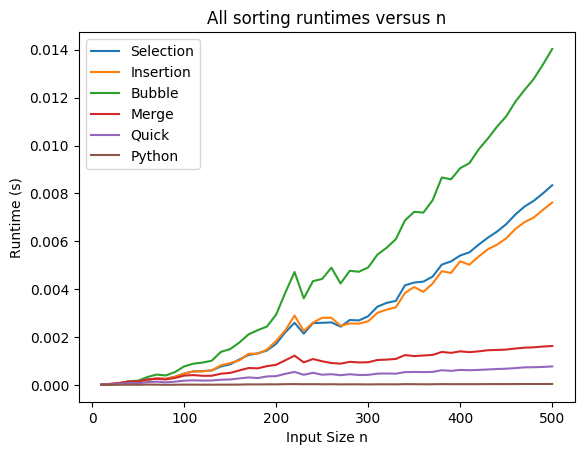
\includegraphics[width = \textwidth]{../results/background}
	\caption{Testing algorithms with expensive computational tasks in the background}
\end{figure}
You will see that the curve goes abnormally: with larger input size, the runtime will sometimes get smaller.

\end{document}